% !TEX root       = ./type_name.tex
% !TEX program    = pdflatex
% !TEX encoding   = utf-8
% !TEX spellcheck = de_DE_frami
%=======================================================================
\chapter{Designing the Application}\label{ch:application_design}
This chapter delves into the design objectives of the application, the architectural frame work of the RYU controller and converting the design into a Python code.

\section{The Design Objectives}

The finished application should be compatible with the RYU controller and be able to handle packets in real time. The timing diagram\ref{fig:Radius-Timing} shows how the RADIUS control flow should happen in the application for authentication.

\subsection{RADIUS Procedure} \label{RADIUS_Procedure}

\begin{figure}
	\centering
	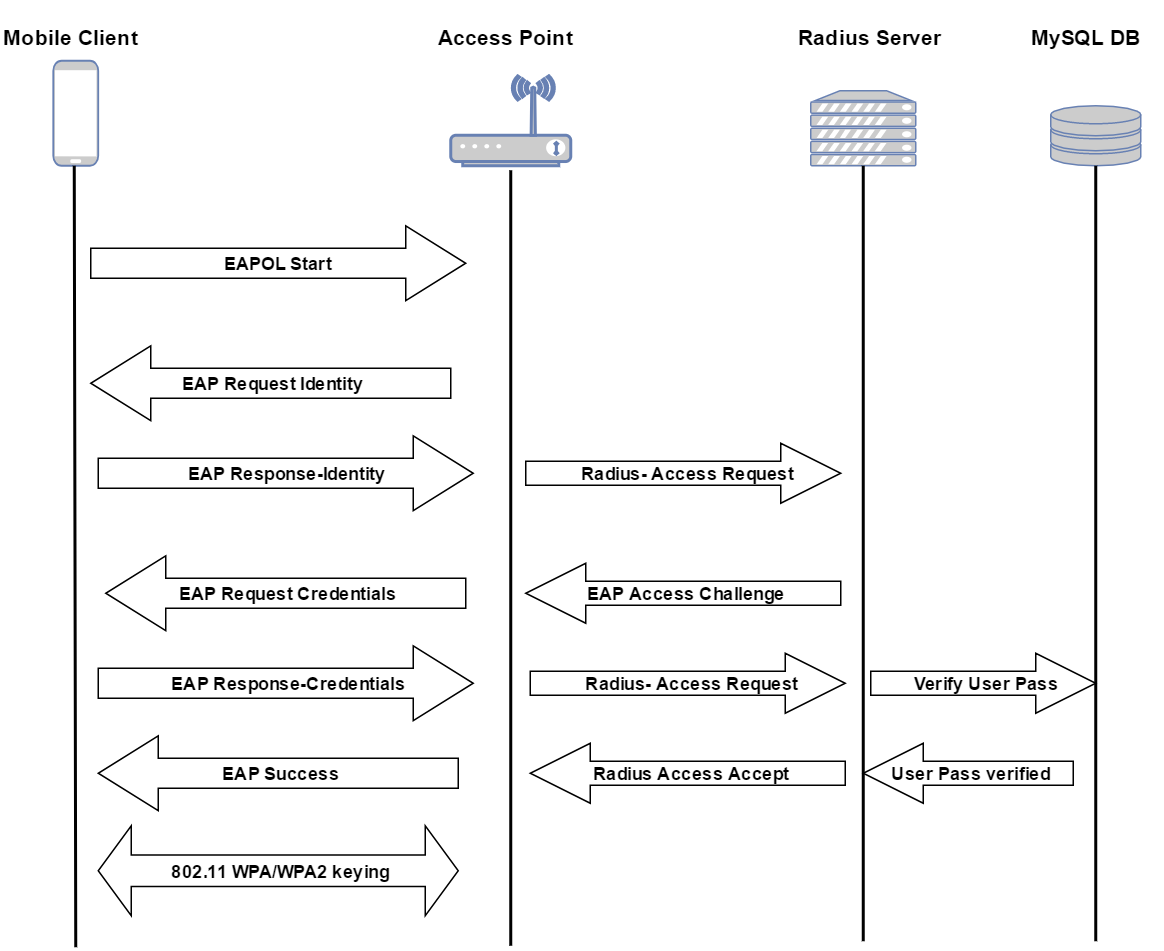
\includegraphics[width=1.0\linewidth]{RADIUS-Timing}
	\caption {RADIUS Authentication Procedure - Timing Diagram }
	\label{fig:Radius-Timing}
	\vspace{-10pt}
\end{figure}

\begin{enumerate}
	\item The mobile client first initiates a radius authentication request with the Access Point.
	\item The packet is verified and authenticated by the RADIUS request and response messages.
	\item If the authentication is a success, the connection is setup with the access point with WPA2 enterprise keying.
	\item Once the client is authenticated, it makes a DHCP request with the access point.   
	
\end{enumerate}
The flowchart \ref{fig:RYU-Flowchart} shows the authentication procedure of the RADIUS server. It also shows the step by step actions that take place in authenticating a client.
\begin{figure}
	\centering
	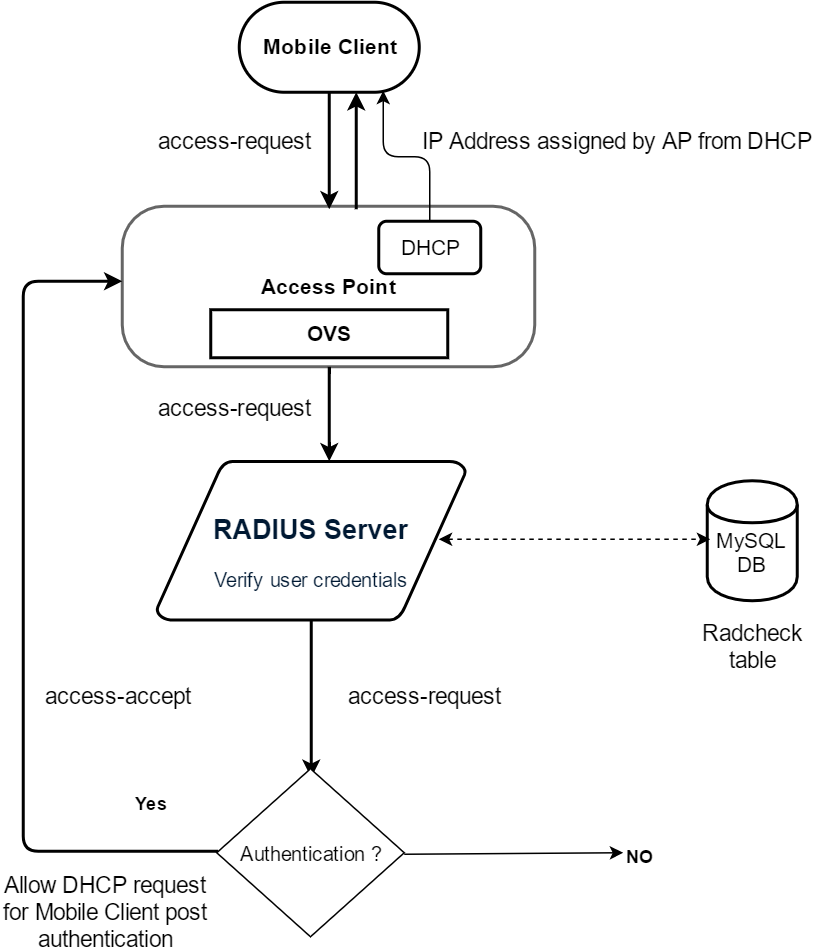
\includegraphics[width=1.0\linewidth]{RADIUS-Flowchart}
	\caption {RADIUS Authentication Procedure - Flowchart }
	\label{fig:Radius-Flowchart}
	\vspace{-10pt}
\end{figure}
\subsection{RYU Control Procedure} \label{RYU Control Procedure}
The timing diagram of RYU \ref{fig:RYU-Timing} shows how the RYU is supposed to listen to the MAC address of the client and parse the packet to assing the destination port id for the client.

\begin{figure}
	\centering
	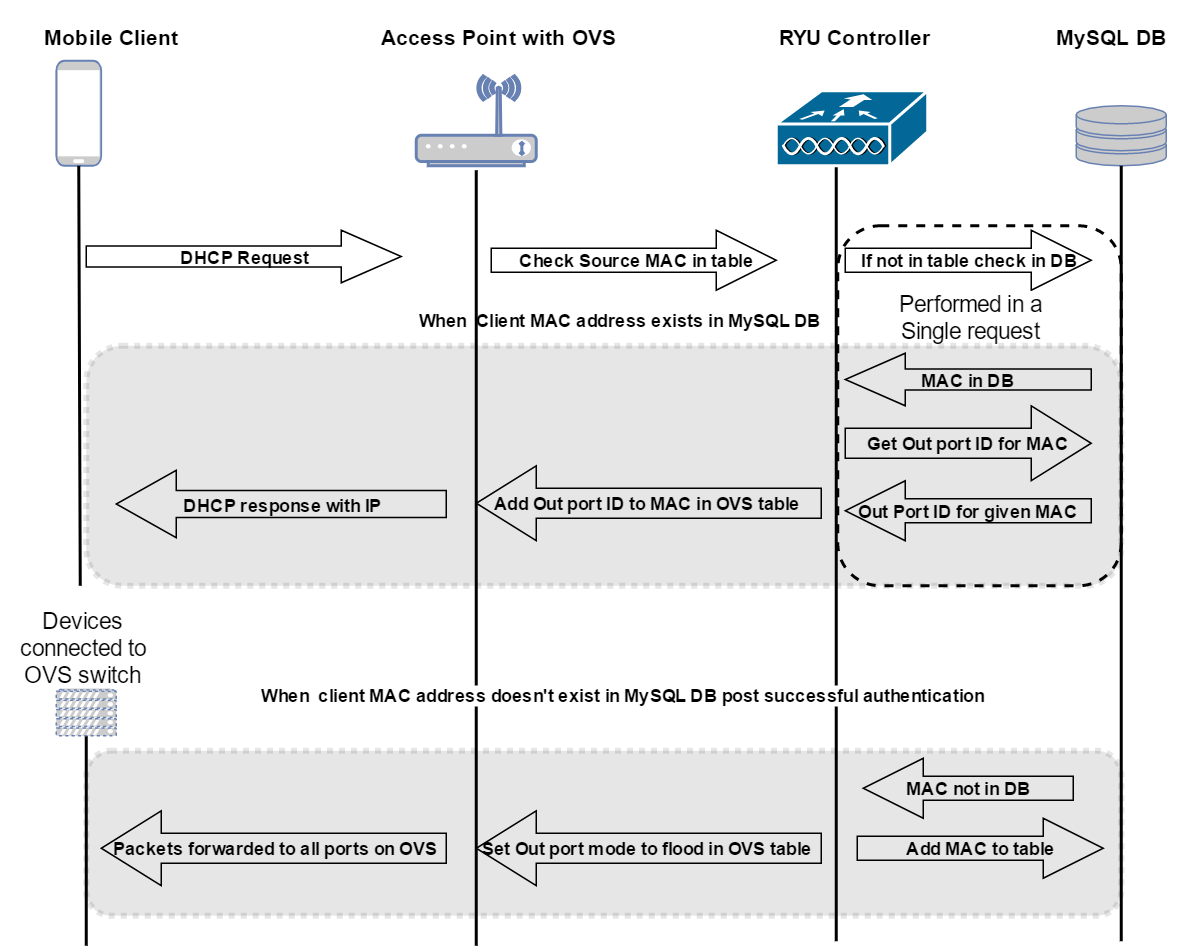
\includegraphics[width=1.0\linewidth]{RYU-Timing}
	\caption {RYU Control Procedure - Timing Diagram }
	\label{fig:RYU-Timing}
	\vspace{-10pt}
\end{figure}

When the client initiates a DHCP request to the access point, the RYU controller listens to the clients MAC address and checks if it exists in the OVS flow table. If it exists, then apply the corresponding rule associated for the MAC address. If it doesn’t exist, then check for the MAC address in the MySQL database. In the first scenario, if the MAC address exists in the MySQL DB, the out port ID associated with the MAC address is retrieved. The retrieved out port id is assigned to the MAC address and an entry is created in the OVS flow table and completes the process with a DHCP response.

In the second scenario after the authentication of the client is successful, if the MAC address does not exist in MySQL DB. The MAC address is added to the table and the out port id is set to flood mode in the OVS flow table in the access point. The process is completed with a DHCP response by providing an IP address to the client. In case of an attack, the system becomes vulnerable only when the fake MAC address used by the client matches with the user credential used for authentication. In such cases a firewall is used to further protect the system.

%\begin{enumerate}
%	\item When the client initiates a DHCP request to the access point, the RYU controller listens to the clients MAC address and checks if it exists in the OVS flow table.
%	\item If it exists, apply the corresponding rule associated with the MAC. If it doesn’t exist, check the MAC in the MySQL database.
%	\item In the first scenario, if the MAC address exists in the MySQL DB, get the port ID associated with the MAC.
%	\item Apply this out port id from the database to the MAC address and add the flow to the OVS flow table and complete the DHCP response.
%	\item In the second scenario, if the MAC address does not exist in MySQL DB, add the MAC to the table and set the port id to flood mode in the OVS flow table in the access point.
%	\item Complete the DHCP response by providing an IP to the client.
%	
%\end{enumerate}
The flowchart  \ref{fig:RYU-Flowchart} will provide an overview of the control flow that would take place in the RYU controller and the OVS. Starting from learning the MAC address to assigning the out port id to the MAC.

\begin{figure}
	\centering
	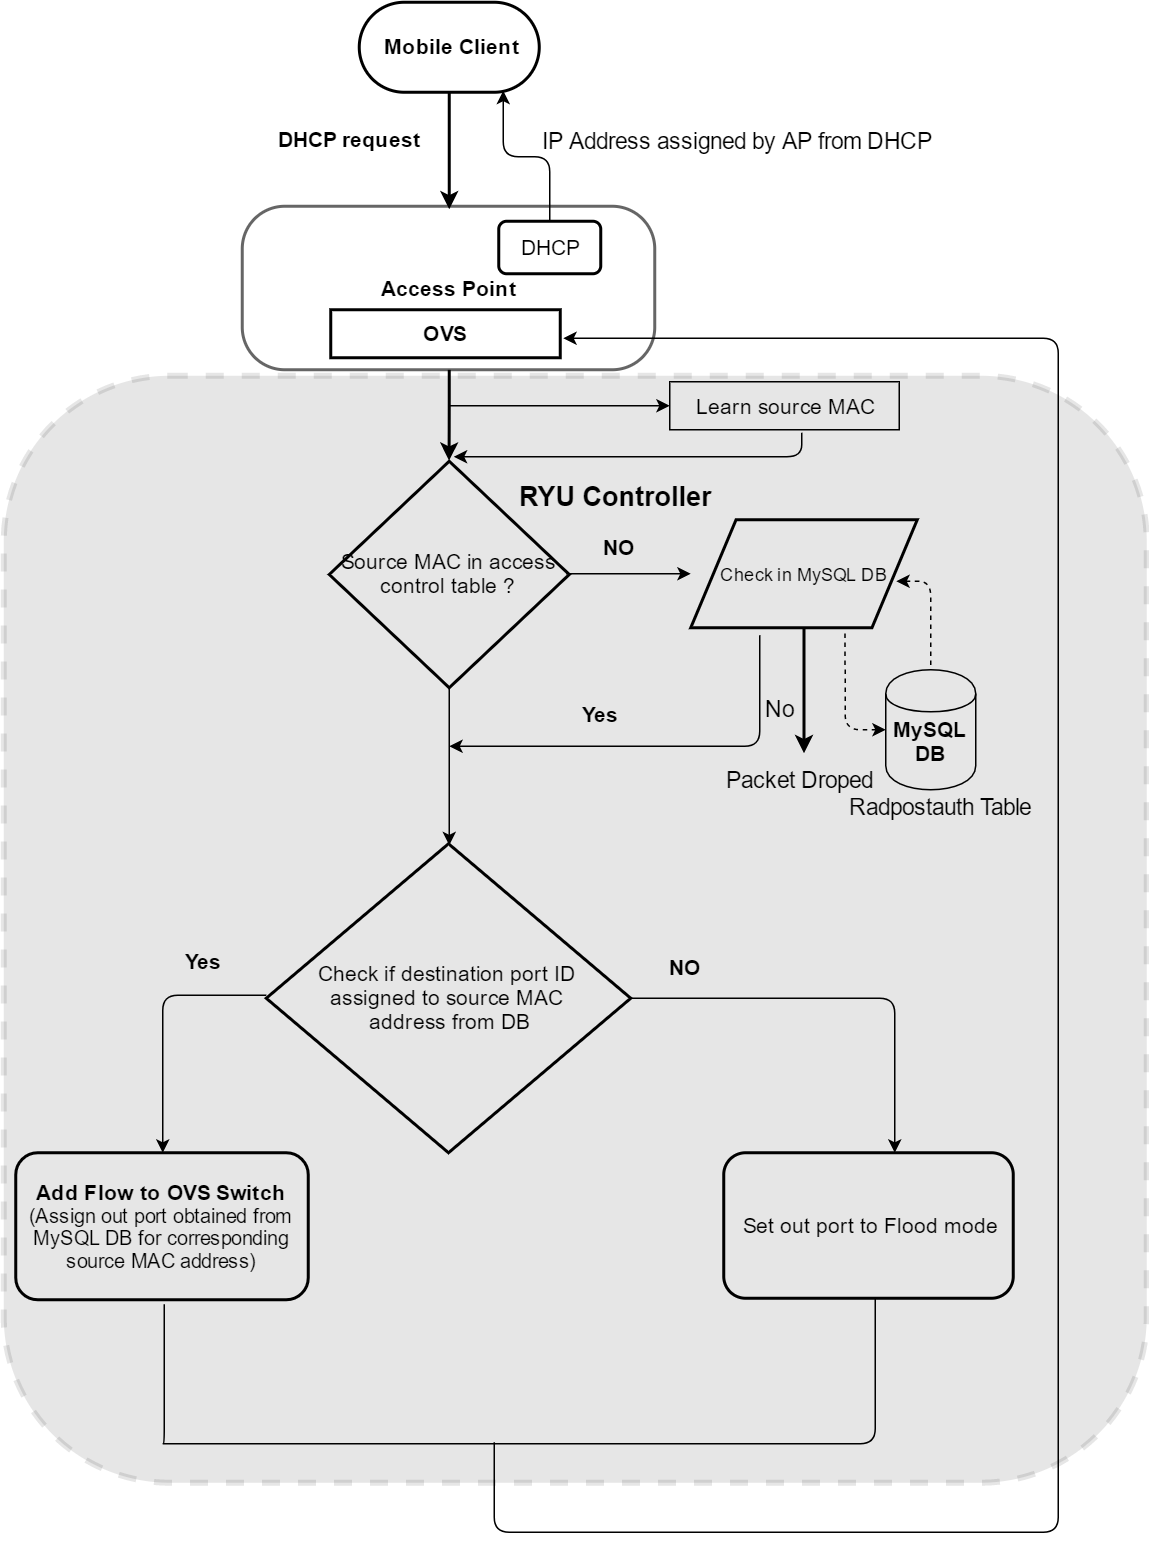
\includegraphics[width=1.0\linewidth]{RYU-Flowchart}
	\caption {RYU Control Procedure - Flowchart}
	\label{fig:RYU-Flowchart}
	\vspace{-10pt}
\end{figure}

From the flowchart \ref{fig:RYU-Flowchart}, it is clear that the initial DHCP request made by the mobile client to the AP is flooded to all ports in the AP. The RYU controller captures this request and retrieves the MAC address of the client. The packet passes through two conditions, the first condition is to check whether the client MAC address is already in the table. If the MAC address exists, then the packet passes to the second condition. The second condition is where the MAC address is checked if it is associated to a corresponding out port ID.  In case, the out port ID is found. Then the packet is converted to a unicast with the assigned out port through which all the packets coming from the client will pass through to its destination in future. If the packet fails in the first condition, then the packet is dropped else if it fails in the second condition. The packet is flooded to all the ports in the OVS and the MAC address is learnt to avoid flooding in future.

Due to the current OpenFlow version (v1.3) used by the OVS, it is limited to assigning only one out port per user instead of multiple ports. This feature will be available in future versions of OpenFlow when supported by OVS.

\section{RYU Manager Process \cite{RYU_app_process}} \label{RYU_Manager_Process}
 For designing the application, the RYU manager process is considered. This is explained using the diagram \ref{fig:RYU-Event-Process}.
 \begin{figure}
 	\centering
 	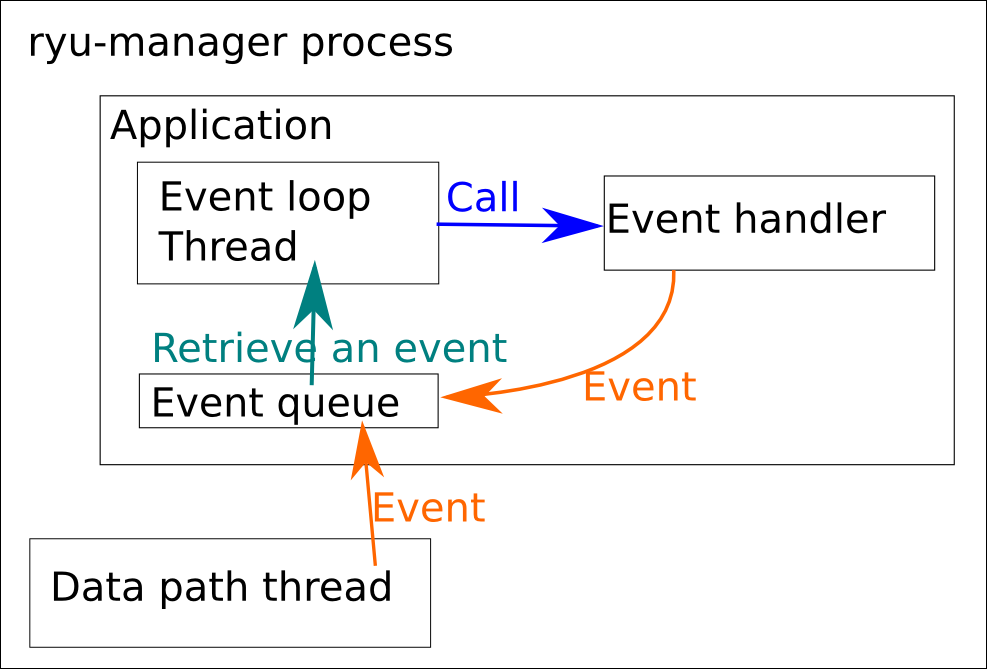
\includegraphics[width=1.0\linewidth]{RYU-event-process}
 	\caption {RYU Manager Event Process \cite{RYU_event_process_diag}}
 	\label{fig:RYU-Event-Process}
 	\vspace{-10pt}
 \end{figure}
To build the application in python, the following classes are mainly used which are explained below.

\begin{itemize}
	\item Application is the user logic that explains how the application should behave. It is a class that inherits the \textit{ryu.base.app\_manager.RyuApp}.
	\item Events are class objects that are used in communication between applications. It inherits the class \textit{ryu.controller.event.EventBase}.
	\item Event queues are the single queues that each application has for receiving events.
	\item RYU uses eventlets to run in multi-threaded environment. These threads are non-preemptive.
	\item Event Loops: A thread that is created for each application runs an event loop. When there is an event in the queue, this loop will load the event and call the corresponding handler.
	\item Event Handlers:  They are user defined handlers designed to handle when a specific type of event occurs. They reside in the event loop of an application. Event handlers can be defined by decorating the application class method with the \textit{ryu.controller.handler.set\_ev\_cls} decorator.
	
\end{itemize}

\section{Python Coding}\label{Python_code}
The code is built using an existing RYU MAC learning application and is modified for user segregation.

The \textit{set\_ev\_class} sets the event handler for packet-in event and passing it on to the method \textit{ \_packet\_in\_handler} to parse the incoming packet. The packet is parsed by the method and details about the packet are extracted such as the in-port, datapath, payload etc.

\begin{lstlisting} [language=Python]
	@set_ev_cls(ofp_event.EventOFPPacketIn, MAIN_DISPATCHER)
	def _packet_in_handler(self, ev):
		# If you hit this you might want to increase
		# the "miss_send_length" of your switch
		if ev.msg.msg_len < ev.msg.total_len:
			self.logger.debug("packet truncated: only %s of %s bytes", ev.msg.msg_len, ev.msg.total_len)
		msg = ev.msg
		datapath = msg.datapath
		ofproto = datapath.ofproto
		parser = datapath.ofproto_parser
		in_port = msg.match['in_port']
		pkt = packet.Packet(msg.data)
		eth = pkt.get_protocols(ethernet.ethernet)[0]
		udp_payload = pkt.get_protocols(udp.udp)
\end{lstlisting}

Once the source and destination MAC address is retrieved from the packet, the source MAC address is then checked in the MySQL DB as shown in the figure above. The statement \textit{cursor.execute} also retrieves the port id from the database for the corresponding MAC if it is found as shown in the code snippet below.

\begin{lstlisting} [language=Python]
	#creating a mysql connection to database
		
	connection = MySQLdb.connect(host = "192.168.1.169", user = "freerad", passwd = "pass", db = "radius")
	cursor = connection.cursor ()
	
	#cursor.execute ("select CallingStationId from radpostauth order by id desc LIMIT 1")
	#data = cursor.fetchall ()
	cursor.execute ("SELECT portid FROM radcheck WHERE username IN (SELECT user FROM radpostauth WHERE CallingStationId = %s AND id = (SELECT MAX(id) from radpostauth) )", src)
	outport_for_src = cursor.fetchone ()
	self.logger.info ("outport_for_src tuple is %s", outport_for_src)
	#portid = outport_for_src[0]
	self.logger.info ("Data is %s", src)	
	cursor.close()
	connection.close ()
	# Mysql verification end
\end{lstlisting}

In this step, the incoming port id (\textit{in\_port}) is stored in the \textit{self.mac\_to\_port} array. The first \textit{if} condition then checks if the destination MAC address is in the array \textit{self.mac\_to\_port}, if it exists then the second condition checks if the out port retrieved form the database is not empty or null. Then the third condition checks if the retrieved out port id from the database is the same as the one retrieved from the packet coming from the client, then the port id in the array \textit{self.mac\_to\_port} is assigned to the \textit{out\_port} variable.

\begin{lstlisting}[language=Python]
	    self.mac_to_port[dpid][src] = in_port

	self.logger.info ("DST is %s", dst)
		if dst in self.mac_to_port[dpid]:
		test = self.mac_to_port[dpid][dst]
		self.logger.info ("self.mac_to_port[dpid][dst] value %s", test)
		self.logger.info ("Out_Port before condition %s", outport_for_src)
		if outport_for_src != None and all(outport_for_src):
			if int(outport_for_src[0]) == self.mac_to_port[dpid][dst]:
				out_port = self.mac_to_port[dpid][dst]
				self.logger.info ("Out_Port is the same as in database table %s", out_port)
			else:
				self.logger.info ("Out_Port is not allowed, dropping packet")	
				return	
		else:
			#except (TypeError,UnboundLocalError):		
			out_port = self.mac_to_port[dpid][dst]		
			self.logger.info ("Out_Port not defined in database, using learned port")	
\end{lstlisting}

The flowing code snipped explains the scenario when there is no out-port id is mentioned in the database for the corresponding MAC address. 

\begin{lstlisting}[language=Python]
	else:
	#except (TypeError,UnboundLocalError):

		out_port = ofproto.OFPP_FLOOD
	#out_port = 4
		self.logger.info ("Out_Port is Flooded %s", out_port)

self.logger.info ("Above actions Out_Port %s", out_port)
	actions = [parser.OFPActionOutput(out_port)]
self.logger.info ("Actions is %s", actions)
\end{lstlisting}

The variable \textit{out\_port} is assigned a FLOOD mode and the parser \textit{parser.OFPActionOutput} is called to parse the \textit{out\_port} mode set in the previous conditions. 

A new flow is then assigned to the OVS switch with the obtained \textit{out\_port} conditions. The code snipped below shows the usual procedure to add the flow by using \textit{add\_flow} method providing values such as datapath, match conditions, and actions like setting the out port and buffer id if it exists. The packet is updated with the new information and sent out using the \textit{send\_msg} method that sends it to the OVS switch and a new flow entry is created in the OVS flow table.

\begin{lstlisting} [language=Python]
		 # install a flow to avoid packet_in next time
		if out_port != ofproto.OFPP_FLOOD:
		self.logger.info ("Out_Port not flooded adding flow ")	
			match = parser.OFPMatch(in_port=in_port, eth_dst=dst)
			#match = parser.OFPMatch(in_port=in_port, eth_dst='a0:f3:c1:77:d8:36')
			# verify if we have a valid buffer_id, if yes avoid to send both
			# flow_mod & packet_out
			if msg.buffer_id != ofproto.OFP_NO_BUFFER:
				self.add_flow(datapath, 1, match, actions, msg.buffer_id)
				return
			else:
				self.add_flow(datapath, 1, match, actions)
		data = None
		if msg.buffer_id == ofproto.OFP_NO_BUFFER:
			data = msg.data	
		out = parser.OFPPacketOut(datapath=datapath, buffer_id=msg.buffer_id, in_port=in_port, actions=actions, data=data)
		datapath.send_msg(out)
\end{lstlisting}